\section{神经网络}
\begin{center}
	\begin{tikzpicture}[
		>=latex,
		neuron/.style={circle, draw, thick, minimum size=6mm, inner sep=0pt},
		conn/.style={-Latex, thick},
		layerlabel/.style={font=\small},
		x=1.8cm, y=1.0cm
		]
		
		% -----------------------------
		% Layer sizes (edit as needed)
		% -----------------------------
		\def\nIn{4}
		\def\nHone{4}
		\def\nHtwo{4}
		\def\nOut{2}
		
		% -----------------------------
		% Input layer
		% -----------------------------
		\foreach \i in {1,...,\nIn} {
			\node[neuron] (I-\i) at (0, -\i) {};
		}
		\node[layerlabel] at (0, 0) {Input};
		
		% -----------------------------
		% Hidden layer 1
		% -----------------------------
		\foreach \j in {1,...,\nHone} {
			\node[neuron] (H1-\j) at (1, -\j) {};
		}
		\node[layerlabel] at (1, 0) {Hidden 1};
		
		% -----------------------------
		% Hidden layer 2
		% -----------------------------
		\foreach \k in {1,...,\nHtwo} {
			\node[neuron] (H2-\k) at (2, -\k) {};
		}
		\node[layerlabel] at (2, 0) {Hidden 2};
		
		% -----------------------------
		% Output layer
		% -----------------------------
		\foreach \m in {1,...,\nOut} {
			\node[neuron] (O-\m) at (3, -\m-1) {};
		}
		\node[layerlabel] at (3, 0) {Output};
		
		% -----------------------------
		% Fully-connected edges
		% -----------------------------
		\foreach \i in {1,...,\nIn} {
			\foreach \j in {1,...,\nHone} {
				\draw[conn] (I-\i) -- (H1-\j);
			}
		}
		\foreach \j in {1,...,\nHone} {
			\foreach \k in {1,...,\nHtwo} {
				\draw[conn] (H1-\j) -- (H2-\k);
			}
		}
		\foreach \k in {1,...,\nHtwo} {
			\foreach \m in {1,...,\nOut} {
				\draw[conn] (H2-\k) -- (O-\m);
			}
		}
	\end{tikzpicture}
\end{center}
\begin{definition}
	若映射$f_\theta:\mathbb{R}^m\rightarrow\mathbb{R}^n$可以表示为若干线性变换与逐元素非线性映射的复合:
	\begin{equation*}
		f_\theta(x)=\phi^{(L)}\!\circ \phi^{(L-1)} \circ \cdots \circ \phi^{(1)}(x)
	\end{equation*}
	其中第$l$层映射$\phi^{(l)}:\mathbb{R}^{n_{l-1}}\to\mathbb{R}^{n_l}$ 定义为:
	\begin{equation*}
		\phi^{(l)}(z)=\sigma^{(l)}\!\left(W^{(l)}z+b^{(l)}\right),\quad l=1,2,\dots,L
	\end{equation*}
	这里:
	\begin{itemize}
		\item $W^{(l)}\in\mathbb{R}^{n_l\times n_{l-1}}$ 为第 $l$ 层的权重矩阵,
		\item $b^{(l)}\in\mathbb{R}^{n_l}$ 为偏置向量,
		\item $\sigma^{(l)}$ 为逐元素作用的非线性函数,
		\item $\theta=\{W^{(l)},b^{(l)}\}_{l=1}^L$ 为网络的全部可学习参数;
	\end{itemize}
	则称$f_\theta$为\gls{NN},非线性映射$\sigma^{(l)}$被称之为\gls{ActivationFunction}。当$L>2$ 时,位于输入层与输出层之间的各层称为\gls{HiddenLayer}。
\end{definition}
\begin{note}
	引入激活函数的原因有两点:
	\begin{enumerate}
		\item 如果网络中所有层都是线性函数,则整个网络表示的是线性模型,增加深度不会提升表达能力(无论增加多少层,总能以一个线性映射来等价表示,即多层神经网络等价于一层)。
		\item 引入非线性函数可以使得模型有能力拟合非线性函数,
	\end{enumerate}
\end{note}
下面给出一些常见的激活函数。
\begin{definition}
	称函数:
	\begin{equation*}
		\sigma(x) = \frac{1}{1+\exp(-x)}
	\end{equation*}
	为\gls{SigmoidFunction}。
\end{definition}
\begin{figure}[H]
	\centering
	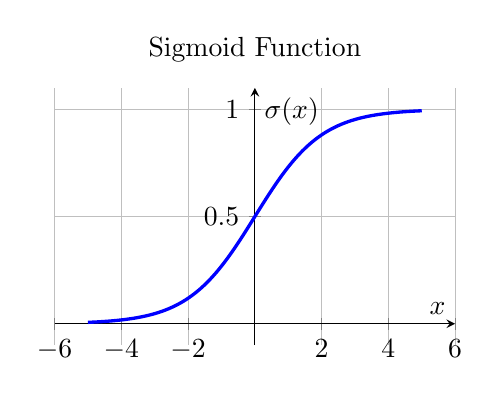
\begin{tikzpicture}
		\begin{axis}[
			width=0.55\textwidth,
			height=0.4\textwidth,
			xmin=-6, xmax=6,
			ymin=-0.1, ymax=1.1,
			axis lines=middle,
			xlabel={$x$},
			ylabel={$\sigma(x)$},
			grid=both,
			samples=200,
			title={Sigmoid Function},
			]
			\addplot[very thick, blue] {1/(1+exp(-x))};
		\end{axis}
	\end{tikzpicture}
	\caption{Sigmoid 激活函数$\sigma(x)=\dfrac{1}{1+e^{-x}}$}
\end{figure}
\begin{definition}
	称函数:
	\begin{equation*}
		\tanh(x)=\frac{e^x - e^{-x}}{e^x + e^{-x}}
	\end{equation*}
	为\gls{TanhFunction}。
\end{definition}
\begin{figure}[H]
	\centering
	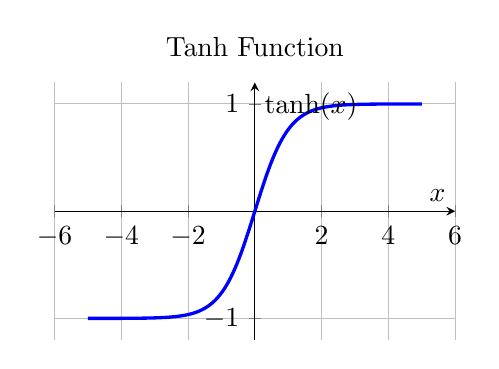
\begin{tikzpicture}
		\begin{axis}[
			width=0.55\textwidth,
			height=0.4\textwidth,
			xmin=-6, xmax=6,
			ymin=-1.2, ymax=1.2,
			axis lines=middle,
			xlabel={$x$},
			ylabel={$\tanh(x)$},
			grid=both,
			samples=200,
			title={Tanh Function},
			]
			\addplot[very thick, blue] {tanh(x)};
		\end{axis}
	\end{tikzpicture}
	\caption{Tanh 激活函数 $\tanh(x)$}
\end{figure}
\begin{definition}
	称函数:
	\begin{equation*}
		\sigma(x)=\max(0,x)
	\end{equation*}
	为\gls{ReLU}。
\end{definition}
\begin{figure}[H]
	\centering
	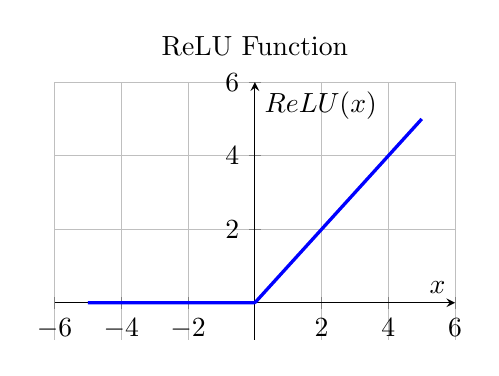
\begin{tikzpicture}
		\begin{axis}[
			width=0.55\textwidth,
			height=0.4\textwidth,
			xmin=-6, xmax=6,
			ymin=-1, ymax=6,
			axis lines=middle,
			xlabel={$x$},
			ylabel={$\operatorname{ReLU}(x)$},
			grid=both,
			samples=200,
			title={ReLU Function},
			]
			\addplot[very thick, blue] {max(0,x)};
		\end{axis}
	\end{tikzpicture}
	\caption{ReLU 激活函数 $\sigma(x)=\max(0,x)$}
\end{figure}
\begin{definition}
	称函数:
	\begin{equation*}
		\sigma(x)=
		\begin{cases}
			x,& x>0 \\
			\alpha x, & x\leqslant 0
		\end{cases}
		\quad (\alpha>0 \text{为较小常数})
	\end{equation*}
	为\gls{LeakyRectifiedLinearUnit}。
\end{definition}
\begin{figure}[H]
	\centering
	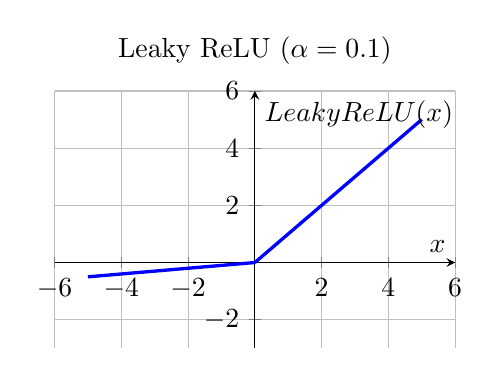
\begin{tikzpicture}
		\begin{axis}[
			width=0.55\textwidth,
			height=0.4\textwidth,
			xmin=-6, xmax=6,
			ymin=-3, ymax=6,
			axis lines=middle,
			xlabel={$x$},
			ylabel={$\operatorname{Leaky ReLU}(x)$},
			grid=both,
			samples=200,
			title={Leaky ReLU ($\alpha=0.1$)},
			]
			\addplot[very thick, blue] {(x>0)*x + (x<=0)*(0.1*x)};
		\end{axis}
	\end{tikzpicture}
	\caption{Leaky ReLU 激活函数($\alpha=0.1$)}
\end{figure}
\begin{definition}
	称函数:
	\begin{equation*}
		\sigma(x)=
		\begin{cases}
			x, & x>0 \\
			\alpha(e^x-1), & x\leqslant 0
		\end{cases}
	\end{equation*}
	为\gls{ELU}。
\end{definition}
\begin{figure}[H]
	\centering
	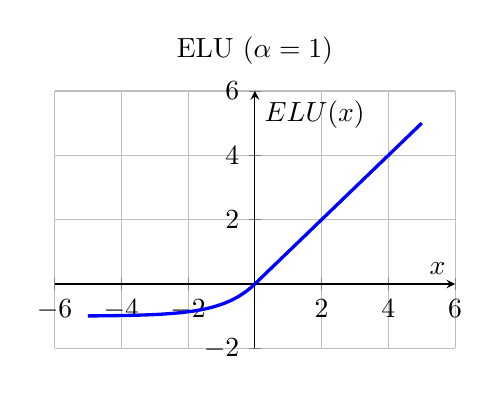
\begin{tikzpicture}
		\begin{axis}[
			width=0.55\textwidth,
			height=0.4\textwidth,
			xmin=-6, xmax=6,
			ymin=-2, ymax=6,
			axis lines=middle,
			xlabel={$x$},
			ylabel={$\operatorname{ELU}(x)$},
			grid=both,
			samples=200,
			title={ELU ($\alpha=1$)},
			]
			\addplot[very thick, blue] {(x>0)*x + (x<=0)*(exp(x)-1)};
		\end{axis}
	\end{tikzpicture}
	\caption{ELU 激活函数($\alpha=1$)}
\end{figure}
\begin{definition}
	设输入向量$z=(\seq{x}{n})^\top$,称映射:
	\begin{equation*}
		\sigma(x)_i=\frac{e^{x_i}}{\sum\limits_{j=1}^ne^{x_j}}, \quad i=1,\dots,n
	\end{equation*}
	为\gls{SoftmaxFunction}。
\end{definition}

\subsection{模型学习}
\subsubsection{损失函数}
\begin{definition}
	设观测样本集为\(\mathcal{D}=\{(x_i,y_i)\}_{i=1}^n\),模型为函数$f_\theta$,记$\hat{y}_i=f_\theta(x_i)$。若函数$L(y,\hat{y})$用于衡量模型预测值与真实值之间差异,则称$L$为\gls{LossFunction}。称:
	\begin{equation*}
		\widehat{\mathcal{R}}(\theta)=\frac{1}{n}\sum_{i=1}^{n}L[y_i,f_\theta(x_i)]
	\end{equation*}
	为\gls{EmpiricalRisk}。
\end{definition}
\subsubsection{梯度下降}
\begin{note}
	设 $f:\mathbb{R}^n\to\mathbb{R}$ 在点$x$处Fr\'echet可微,任取单位向量$u\in\mathbb{R}^n$,由\cref{prop:FrechetGateaux}(1)可知$f$在方向$u$上的方向导数为$\dif f(x;u)=(\operatorname{D}fx)h$,由\cref{ineq:cauchy-ineq-R}可得:
	\begin{equation*}
		\dif f(x;u)=(\operatorname{D}fx)h\leqslant||\operatorname{D}fx||\;||h||=||\operatorname{D}fx||
	\end{equation*}
	上式取等当且仅当$u$与$\operatorname{D}fx$同方向。  \par
	因此,在所有单位方向中,函数在方向$\operatorname{D}fx$上的方向导数取得最大值,即函数在点$x$处沿梯度方向上升最快,而沿$-\operatorname{D}fx$方向下降最快。
\end{note}
\begin{definition}
	\gls{GradientDescent}指的是:在最小化目标函数$f$的优化问题中,每次迭代过程为在当前点$x_t$处沿负梯度方向$-\operatorname{D}f(x_t)$移动一小步。
\end{definition}
\begin{definition}
	称正数$\eta>0$为\gls{LR}。 
\end{definition}
\begin{note}
	在第$t$次迭代中,参数更新通常写为:
	\begin{equation*}
		\theta_{t+1}=\theta_t-\eta g_t
	\end{equation*}
	其中$g_t$为当前点处目标函数关于参数$\theta$的梯度估计。\par
	学习率决定了参数更新的幅度:$\eta$过大会导致算法发散或震荡,$\eta$过小则会使收敛速度显著变慢。
\end{note}
\begin{definition}
	设训练集为$\mathcal{D}=\{(x_i,y_i)\}_{i=1}^n$。称$\mathcal{B}\subseteq\mathcal{D}$为一个\gls{Batch},$|\mathcal{B}|$被称作\gls{BatchSize}。
\end{definition}
\begin{definition}
	称对整个训练集$\mathcal{D}$完整遍历一次的过程为一\gls{Epoch}。
\end{definition}
\begin{algorithm}[H]
	\caption{Batch Gradient Descent}
	\begin{algorithmic}[1]
		\State \textbf{Input:} initial parameter $\theta_0$, learning rate $\eta$, number of iterations $T$, training set $\mathcal{D}$
		\For{$t = 1,2,\dots,T$}
		\State Compute the empirical risk $\widehat{\mathcal{R}}(\theta_t)$ on the whole dataset $\mathcal{D}$
		\State Compute the full gradient $g_t=\dif\widehat{\mathcal{R}}(\theta_t)$
		\State Update the parameter:
		\begin{equation*}
			\theta_{t+1} \gets \theta_t - \eta\, g_t
		\end{equation*}
		\EndFor
		\State \textbf{Return:} final parameter estimate $\theta_T$
	\end{algorithmic}
\end{algorithm}
\begin{algorithm}[H]
	\caption{Stochastic Gradient Descent (SGD)}
	\begin{algorithmic}[1]
		\State \textbf{Input:} initial parameter $\theta_0$, learning rate $\eta$, number of iterations $T$, training set $\mathcal{D}=\{(x_i,y_i)\}_{i=1}^n$
		\For{$t = 1,2,\dots,T$}
		\State Randomly sample one data point $(x_{i_t}, y_{i_t})$ from $\mathcal{D}$
		\State Compute the stochastic gradient
		\[
		g_t = \dif L[f(x_{i_t};\theta_t), y_{i_t}]
		\]
		\State Update the parameter:
		\[
		\theta_{t+1} \gets \theta_t - \eta\, g_t
		\]
		\EndFor
		\State \textbf{Return:} final parameter estimate $\theta_T$
	\end{algorithmic}
\end{algorithm}
\begin{algorithm}[H]
	\caption{Mini-batch Gradient Descent}
	\begin{algorithmic}[1]
		\State \textbf{Input:} initial parameter $\theta_0$, learning rate $\eta$, number of iterations $T$, training set $\mathcal{D}$, batch size $B$
		\For{$t = 1,2,\dots,T$}
		\State Randomly sample a mini-batch $\mathcal{B}_t \subseteq \mathcal{D}$ with $|\mathcal{B}_t| = B$
		\State Compute the mini-batch gradient
		\[
		g_t = \frac{1}{B} \sum_{(x_i,y_i)\in \mathcal{B}_t}
		\dif L[f(x_i;\theta_t), y_i]
		\]
		\State Update the parameter:
		\[
		\theta_{t+1} \gets \theta_t - \eta\, g_t
		\]
		\EndFor
		\State \textbf{Return:} final parameter estimate $\theta_T$
	\end{algorithmic}
\end{algorithm}

\subsection{序列网络}
\subsubsection{循环神经网络(Recurrent Neural Network, RNN)}
\begin{figure}[H]
	\centering
	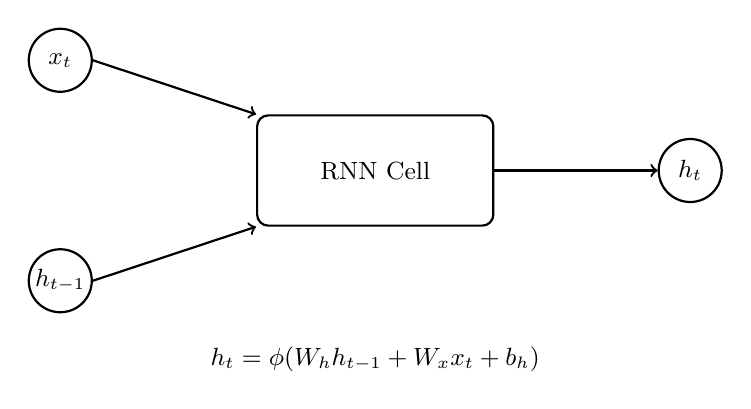
\begin{tikzpicture}[
		font=\small,
		arrow/.style={->, thick},
		state/.style={circle, draw, thick, minimum size=8mm, inner sep=0pt},
		block/.style={rectangle, draw, thick, rounded corners=4pt,
			minimum width=3.0cm, minimum height=1.4cm, align=center}
		]
		
		% ---- Column 1: inputs and previous state ----
		\node[state] (x)     at (0,  1.4) {$x_t$};
		\node[state] (hprev) at (0, -1.4) {$h_{t-1}$};
		
		% ---- Column 2: RNN cell ----
		\node[block] (rnn) at (4, 0) {RNN Cell};
		
		% ---- Column 3: current hidden state (aligned horizontally) ----
		\node[state] (ht) at (8, 0) {$h_t$};
		
		% ---- Equations ----
		\node at (4, -2.4)
		{$h_t=\phi\!\left(W_h h_{t-1}+W_x x_t+b_h\right)$};
		
		% ---- Arrows (clean geometry) ----
		% x_t -> top-left corner of RNN
		\draw[arrow] (x.east) -- (rnn.north west);
		
		% h_{t-1} -> bottom-left corner of RNN
		\draw[arrow] (hprev.east) -- (rnn.south west);
		
		% RNN -> h_t (straight horizontal)
		\draw[arrow] (rnn.east) -- (ht.west);
	\end{tikzpicture}
	\caption{单个时间步的RNN单元计算结构}
\end{figure}
\begin{figure}[H]
	\centering
	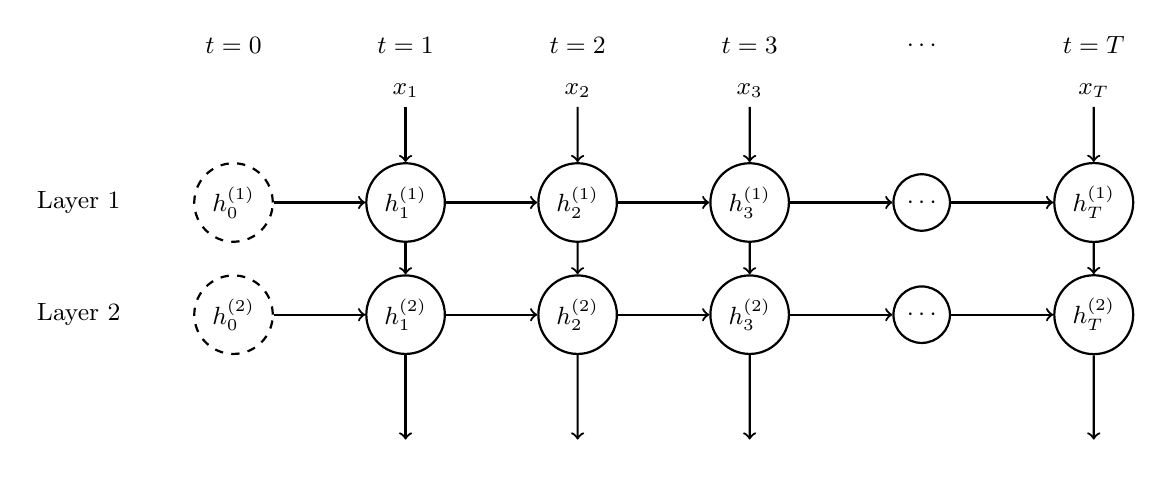
\begin{tikzpicture}[
		scale=0.95,
		every node/.style={font=\small},
		state/.style={circle, draw, thick, minimum size=7mm},
		state0/.style={circle, draw, thick, dashed, minimum size=7mm},
		arrow/.style={->, thick},
		x=2.3cm, y=1.5cm
		]
		
		% Time labels
		\node at (-1,2.4) {$t=0$};
		\node at (0,2.4) {$t=1$};
		\node at (1,2.4) {$t=2$};
		\node at (2,2.4) {$t=3$};
		\node at (3,2.4) {$\cdots$};
		\node at (4,2.4) {$t=T$};
		
		% -------- Initial hidden states --------
		\node[state0] (h10) at (-1,1) {$h^{(1)}_0$};
		\node[state0] (h20) at (-1,0) {$h^{(2)}_0$};
		
		% -------- Layer 1 hidden states --------
		\node[state] (h11) at (0,1) {$h^{(1)}_1$};
		\node[state] (h12) at (1,1) {$h^{(1)}_2$};
		\node[state] (h13) at (2,1) {$h^{(1)}_3$};
		\node[state] (h1d) at (3,1) {$\cdots$};
		\node[state] (h1T) at (4,1) {$h^{(1)}_T$};
		
		% -------- Layer 2 hidden states --------
		\node[state] (h21) at (0,0) {$h^{(2)}_1$};
		\node[state] (h22) at (1,0) {$h^{(2)}_2$};
		\node[state] (h23) at (2,0) {$h^{(2)}_3$};
		\node[state] (h2d) at (3,0) {$\cdots$};
		\node[state] (h2T) at (4,0) {$h^{(2)}_T$};
		
		% -------- Inputs --------
		\node (x1) at (0,2) {$x_1$};
		\node (x2) at (1,2) {$x_2$};
		\node (x3) at (2,2) {$x_3$};
		\node (xT) at (4,2) {$x_T$};
		
		% -------- Outputs --------
		\node (y1) at (0,-1.2) {};
		\node (y2) at (1,-1.2) {};
		\node (y3) at (2,-1.2) {};
		\node (yT) at (4,-1.2) {};
		
		% ---- Temporal connections (layer 1) ----
		\draw[arrow] (h10) -- (h11);
		\draw[arrow] (h11) -- (h12);
		\draw[arrow] (h12) -- (h13);
		\draw[arrow] (h13) -- (h1d);
		\draw[arrow] (h1d) -- (h1T);
		
		% ---- Temporal connections (layer 2) ----
		\draw[arrow] (h20) -- (h21);
		\draw[arrow] (h21) -- (h22);
		\draw[arrow] (h22) -- (h23);
		\draw[arrow] (h23) -- (h2d);
		\draw[arrow] (h2d) -- (h2T);
		
		% ---- Vertical connections (between layers) ----
		\draw[arrow] (h11) -- (h21);
		\draw[arrow] (h12) -- (h22);
		\draw[arrow] (h13) -- (h23);
		\draw[arrow] (h1T) -- (h2T);
		
		% ---- Input to first layer ----
		\draw[arrow] (x1) -- (h11);
		\draw[arrow] (x2) -- (h12);
		\draw[arrow] (x3) -- (h13);
		\draw[arrow] (xT) -- (h1T);
		
		% ---- Second layer to output ----
		\draw[arrow] (h21) -- (y1);
		\draw[arrow] (h22) -- (y2);
		\draw[arrow] (h23) -- (y3);
		\draw[arrow] (h2T) -- (yT);
		
		% Layer labels
		\node[left] at (-1.6,1) {Layer 1};
		\node[left] at (-1.6,0) {Layer 2};
		
	\end{tikzpicture}
	\caption{循环神经网络结构示意图}
\end{figure}
\begin{algorithm}[H]
	\caption{Forward Propagation of a Multi-layer RNN}
	\label{alg:stacked_rnn_forward}
	\begin{algorithmic}[1]
		
		\Require 
		Input sequence $\{x_t^{(1)}\}_{t=1}^T$, 
		parameters $\{W_h^{(l)}, W_x^{(l)}, b_h^{(l)}\}_{l=1}^{L}$, 
		activation functions $\phi(\cdot)$
		
		\Ensure 
		Hidden states $\{h_t^{(l)}\}_{l=1}^{L}$
		\State Initialize hidden states $h_0^{(l)} = \mathbf{0}$ for all $l = 1,\dots,L$
		\For{$t = 1$ \textbf{to} $T$}   \Comment{Iterate over time steps}
		\For{$l= 1$ \textbf{to} $L$}  \Comment{Iterate over layers}
		\If{$l\ne1$}
		\State $x_t^{(l)} \gets h_t^{(l-1)}$
		\Comment{Output of previous layer as current input}
		\EndIf
		\State $h_t^{(l)} 
		\gets 
		\phi\left(
		W_h^{(l)} h_{t-1}^{(l)} 
		+ 
		W_x^{(l)} x_t^{(l)} 
		+ 
		b_h^{(l)}
		\right)$
		\EndFor
		\EndFor
	\end{algorithmic}
\end{algorithm}
\begin{note}
由于隐藏状态不断累积先前信息,RNN 能够捕捉序列中的依赖关系。
\end{note}
\subsubsection{长短期记忆网络(Long Short-Term Memory, LSTM)}
\begin{algorithm}[H]
	\caption{Forward Propagation of a Multi-layer LSTM}
	\label{alg:stacked_lstm_forward}
	\begin{algorithmic}[1]
		
		\Require 
		Input sequence $\{x_t^{(1)}\}_{t=1}^T$, 
		parameters $\{W_f^{(l)},W_i^{(l)},W_c^{(l)},W_o^{(l)},b_f^{(l)},b_i^{(l)},b_c^{(l)},b_o^{(l)}\}_{l=1}^{L}$
		
		\Ensure 
		Hidden states $\{h_t^{(l)}\}_{l=1}^{L}$ and cell states $\{c_t^{(l)}\}_{l=1}^{L}$
		
		\State Initialize $h_0^{(l)}=\mathbf{0},\; c_0^{(l)}=\mathbf{0}$ for all $l=1,\dots,L$
		
		\For{$t=1$ \textbf{to} $T$}  
		\Comment{Iterate over time steps}
		
		\For{$l=1$ \textbf{to} $L$}  
		\Comment{Iterate over layers}
		
		\If{$l\ne 1$}
		\State $x_t^{(l)} \gets h_t^{(l-1)}$
		\Comment{Input from the previous layer}
		\EndIf
		
		\State Forget gate: controls how much of $c_{t-1}^{(l)}$ is retained
		\begin{equation*}
			f_t^{(l)} \gets \sigma\!\left(W_f^{(l)}[h_{t-1}^{(l)},x_t^{(l)}]+b_f^{(l)}\right)
		\end{equation*}
		
		\State Input gate: controls how much new information is written
		\begin{equation*}
			i_t^{(l)} \gets \sigma\!\left(W_i^{(l)}[h_{t-1}^{(l)},x_t^{(l)}]+b_i^{(l)}\right)
		\end{equation*}
		
		\State Candidate cell state: new content to be added
		\begin{equation*}
			\tilde c_t^{(l)} \gets \tanh\!\left(W_c^{(l)}[h_{t-1}^{(l)},x_t^{(l)}]+b_c^{(l)}\right)
		\end{equation*}
		
		\State Cell state update: forget old + write new
		\begin{equation*}
			c_t^{(l)} \gets f_t^{(l)}\odot c_{t-1}^{(l)} + i_t^{(l)}\odot \tilde c_t^{(l)}
		\end{equation*}
		
		\State Output gate: controls exposure of cell state
		\begin{equation*}
			o_t^{(l)} \gets \sigma\!\left(W_o^{(l)}[h_{t-1}^{(l)},x_t^{(l)}]+b_o^{(l)}\right)
		\end{equation*}
		
		\State Hidden state: gated and activated cell state
		\begin{equation*}
			h_t^{(l)} \gets o_t^{(l)}\odot \tanh(c_t^{(l)})
		\end{equation*}
		\EndFor
		\EndFor
	\end{algorithmic}
\end{algorithm}
\begin{note}
	在LSTM中,由于sigmoid函数的值域为$(-1,1)$,遗忘门、输入门、输出门分别给出了要对过往信息遗忘的比例、输入信息以往的比例、当前记忆输出的比例。而候选记忆与输出阶段采用 $\tanh$,则是为了将内部状态压缩到有界且零中心的区间 $(-1,1)$,使得无论时间步有多长,内部状态都在一定范围之内,既保证了数值稳定性,又维持良好的梯度传播性质。\par
	这种“线性记忆通道 + 门控比例调节 + 有界非线性输出”的结构,使得 LSTM 能够在长时间尺度上同时实现稳定记忆存储与灵活信息选择,是其优于普通RNN的核心原因。
\end{note}
\subsubsection{门控循环单元(Gated Recurrent Unit, GRU)}
\begin{algorithm}[H]
	\caption{Forward Propagation of a Multi-layer GRU}
	\label{alg:stacked_gru_forward}
	\begin{algorithmic}[1]
		
		\Require 
		Input sequence $\{x_t^{(1)}\}_{t=1}^T$, 
		parameters $\{W_z^{(l)},W_r^{(l)},W_h^{(l)},b_z^{(l)},b_r^{(l)},b_h^{(l)}\}_{l=1}^{L}$
		
		\Ensure 
		Hidden states $\{h_t^{(l)}\}_{l=1}^{L}$
		
		\State Initialize $h_0^{(l)}=\mathbf{0}$ for all $l=1,\dots,L$
		
		\For{$t=1$ \textbf{to} $T$}  
		\Comment{Iterate over time steps}
		
		\For{$l=1$ \textbf{to} $L$}  
		\Comment{Iterate over layers}
		
		\If{$l\ne 1$}
		\State $x_t^{(l)} \gets h_t^{(l-1)}$
		\Comment{Input from the previous layer}
		\EndIf
		
		\State Update gate: controls how much of the past state is retained
		\begin{equation*}
			z_t^{(l)} \gets \sigma\!\left(W_z^{(l)}[h_{t-1}^{(l)},x_t^{(l)}]+b_z^{(l)}\right)
		\end{equation*}
		
		\State Reset gate: controls how much past information is ignored
		\begin{equation*}
			r_t^{(l)} \gets \sigma\!\left(W_r^{(l)}[h_{t-1}^{(l)},x_t^{(l)}]+b_r^{(l)}\right)
		\end{equation*}
		
		\State Candidate hidden state: new content to be written
		\begin{equation*}
			\tilde h_t^{(l)} \gets \tanh\!\left(W_h^{(l)}[r_t^{(l)}\odot h_{t-1}^{(l)},x_t^{(l)}]+b_h^{(l)}\right)
		\end{equation*}
		
		\State Hidden state update: interpolate between old and new
		\begin{equation*}
			h_t^{(l)} \gets (1-z_t^{(l)})\odot h_{t-1}^{(l)} + z_t^{(l)}\odot \tilde h_t^{(l)}
		\end{equation*}
		\EndFor
		\EndFor
	\end{algorithmic}
\end{algorithm}
\begin{note}
	与LSTM不同,GRU通过将细胞状态与隐藏状态合并为单一状态 $h_t$,并仅引入更新门与重置门对信息流进行控制,从而在保持长期依赖建模能力的同时,显著简化了模型结构与参数规模,但在表达能力与长期记忆精细控制方面略逊于LSTM。
\end{note}

\subsection{图像网络}
在计算机中,一幅图像本质上是一个规则网格上的数值函数。首先将连续的平面区域离散化为一个由$H\times W$个小方格组成的网格,每一个小方格称为一个\gls{Pixel},有序对$(H,W)$称为图像的\gls{SpatialResolution}。像素是图像的最小空间单位,其空间位置通常用整数坐标$(p,q)$表示,其中$p=1,2,\dots,H,\;q=1,2,\dots,W$。因此,一幅分辨率为$H\times W$的图像可以看作在离散网格 $\{1,2,\dots,H\}\times\{1,2,\dots,W\}$ 上定义的数值函数。\par
对于灰度图像(就是黑白图片)而言,每个像素仅对应一个实数,用来描述该位置的强度。灰度强度刻画了该像素“有多亮”或“有多暗”,通常取值在某个区间内,例如:
\begin{equation*}
	I_{p,q} \in [0,255] \quad \text{或} \quad I_{p,q} \in [0,1]
\end{equation*}
其中数值越大表示亮度越高,数值越小表示亮度越低。这样,一幅灰度图像可以用一个矩阵$I\in M_{H\times W}(\mathbb{R}^{})$来表示。\par
对于彩色图像,每个像素不仅具有亮度信息,还包含颜色信息。计算机中最常用的颜色表示方式是RGB模型,即用红色(Red)、绿色(Green)与蓝色(Blue)三种基色的强度线性组合来表示任意颜色。对应地,每一个像素不再是一个标量,而是一个三维向量,这三个分量分别称为三个\gls{Channel},表示该像素在R、G、B三种基色上的强度大小。\par
设图像的空间分辨率为$H\times W$,则一幅RGB彩色图像可以表示为一个三维张量:
\begin{equation*}
	I=(I_{p,q,c})\in\mathbb{R}^{H\times W\times3}
\end{equation*}
其中$(p,q)$表示像素的空间位置,$c\in\{1,2,3\}$分别对应红、绿、蓝三个颜色通道,$I_{p,q,c}$表示位于位置$(p,q)$的像素在第$c$个通道上的\textbf{灰度强度},即该颜色分量的亮度大小。\par
从矩阵的角度看,一幅彩色图像等价于三张大小为$H\times W$的灰度图像在通道维度上的叠加:
\begin{equation*}
	I=\big(I^{(R)},I^{(G)},I^{(B)}\big)
\end{equation*}
其中:
\begin{equation*}
	I^{(R)},I^{(G)},I^{(B)}\in\mathbb{R}^{H\times W}
\end{equation*}
分别表示红色通道、绿色通道与蓝色通道对应的灰度矩阵。\par
换言之,像素刻画\textbf{空间位置},灰度强度刻画\textbf{亮度大小},通道刻画\textbf{颜色分量}。
\subsubsection{卷积}
\begin{definition}
	设输入图像为$X\in M_{H\times W}(\mathbb{R}^{})$。在图像的每一个空间位置$(i,j)$,取其邻域窗口:
	\begin{equation*}
		\{(i+u-1,\; j+v-1) : u=1,\dots,h,\; v=1,\dots,w\}
	\end{equation*}
	并对该邻域内的像素值施加一组固定权重$K=(K_{u,v})\in M_{h\times w}(\mathbb{R}^{})$,定义局部加权求和
	\begin{equation*}
		S_{i,j}=\sum_{u=1}^h\sum_{v=1}^wK_{u,v}X_{i+u-1,j+v-1}
	\end{equation*}	
	由此在整个空间网格上得到的二维数组$S=(S_{i,j})$称为由该局部加权算子产生的\gls{FeatureMap}。
\end{definition}
\begin{definition}
	称矩阵$K=(K_{u,v})\in M_{h\times w}(\mathbb{R}^{})$为\gls{ConvolutionKernel}。
\end{definition}
\begin{figure}[htbp]
	\centering
	\begin{tikzpicture}[scale=0.85]
		
		% ========= 输入 5x5 =========
		\foreach \i in {0,...,4} {
			\foreach \j in {0,...,4} {
				\draw[gray] (\j,\i) rectangle ++(1,1);
			}
		}
		\node at (2.5,5.8) {\small 输入特征图 $X\in\mathbb{R}^{5\times 5}$};
		
		% 三个 3x3 窗口:左上/中间/右下
		\fill[blue!20]   (0,2) rectangle (3,5);
		\draw[thick,blue] (0,2) rectangle (3,5);
		
		\fill[green!20] (1,1) rectangle (4,4);
		\draw[thick,green!70!black] (1,1) rectangle (4,4);
		
		\fill[red!20]   (2,0) rectangle (5,3);
		\draw[thick,red] (2,0) rectangle (5,3);
		
		\node at (2.5,-0.8) {\small 不同位置的 $3\times 3$ 卷积窗口(滑动)};
		
		% ========= 输出 3x3 =========
		\begin{scope}[xshift=9cm]
			\foreach \i in {0,...,2} {
				\foreach \j in {0,...,2} {
					\draw[gray] (\j,\i) rectangle ++(1,1);
				}
			}
			\node at (1.5,3.8) {\small 输出特征图 $Y\in\mathbb{R}^{3\times 3}$};
			
			% 三个对应输出像素:左上/中心/右下
			\fill[blue!20]   (0,2) rectangle ++(1,1);
			\draw[thick,blue] (0,2) rectangle ++(1,1);
			
			\fill[green!20]  (1,1) rectangle ++(1,1);
			\draw[thick,green!70!black] (1,1) rectangle ++(1,1);
			
			\fill[red!20]    (2,0) rectangle ++(1,1);
			\draw[thick,red]  (2,0) rectangle ++(1,1);
		\end{scope}
		
		% ========= 关键:用“中心点 -> 中心点”画箭头(保证对准) =========
		% 输入窗口中心
		\coordinate (inB) at ($(0,2)!0.5!(3,5)$);
		\coordinate (inG) at ($(1,1)!0.5!(4,4)$);
		\coordinate (inR) at ($(2,0)!0.5!(5,3)$);
		
		% 输出像素中心(注意已 xshift=9cm)
		\coordinate (outB) at ($(9cm,0) + (0.5,2.5)$);
		\coordinate (outG) at ($(9cm,0) + (1.5,1.5)$);
		\coordinate (outR) at ($(9cm,0) + (2.5,0.5)$);
		
		% 为了避免箭头穿过输出方块,可把终点稍微往左移一点
		\draw[->,thick,blue]               (inB) -- ($(outB)+(-0.15,0)$);
		\draw[->,thick,green!70!black]     (inG) -- ($(outG)+(-0.15,0)$);
		\draw[->,thick,red]                (inR) -- ($(outR)+(-0.15,0)$);
		
		% ========= 公式 =========
		\node[align=center] at (2.5,-2.2) {\small
			$Y_{i,j}=\displaystyle\sum_{u=1}^{3}\sum_{v=1}^{3}K_{u,v}\,X_{i+u-1,\,j+v-1}$
		};
		
	\end{tikzpicture}
	\caption{二维离散卷积的滑动窗口与输出位置对应关系示意图}
\end{figure}
\begin{note}
	特征图可以理解为:由原始图像通过某种局部加权求和得到的新的二维图像,其每个像素表示某种“特征”的强弱。
\end{note}
\subsubsection{池化}
\begin{definition}
	设输入特征图为$X \in M_{H \times W}(\mathbb{R})$。给定窗口尺寸$(h,w)$以及步幅$(s_h, s_w)$。在输出位置$(i,j)$处,取像素空间位置邻域窗口:
	\begin{equation*}
		W_{i,j}=\bigl\{\, (\, (i-1)s_h + u,\; (j-1)s_w + v \,) :
		u=1,\dots,h,\; v=1,\dots,w \,\bigr\}
	\end{equation*}
	并在该邻域内对像素值施加一个映射$P:\mathbb{R}^{h\times w}\to \mathbb{R}$,称$P$为\gls{PoolingOperator},该操作称为\gls{Poolig}。
\end{definition}
\begin{note}
	卷积只能是局部加权,其主要作用为特征提取与线性滤波,通过可学习权重检测局部模式,而池化则对应着一般的函数,功能为空间降采样。\par
	常见池化函数有:
	\begin{enumerate}
		\item \textbf{最大池化}:在窗口内取最大值。
		\item \textbf{平均池化}:在窗口内取均值。
	\end{enumerate}
\end{note}
\subsubsection{填充}
在上述卷积与池化定义中,邻域窗口$W_{i,j}$可能在靠近边界时超出输入特征图$X$的定义域。为使边界位置也能应用同样的局部算子,通常在输入矩阵四周引入\gls{padding}。在卷积与池化中,所有邻域窗口$W_{i,j}$实际均作用在扩展特征图$\tilde{X}$上。